\documentclass[11pt]{scrartcl}

\usepackage[sexy]{evan}
\usepackage{import}
\usepackage[table]{xcolor}
\usepackage{xfp}
\usepackage{multicol}

\newcommand{\gad}{\textcolor{yellow}{$\bigstar$}}
\newcommand{\bad}{\textcolor{red}{$\bigstar$}}

\definecolor{dcol0}{HTML}{C8E6C9}
\definecolor{dcol1}{HTML}{D4E9B3}
\definecolor{dcol2}{HTML}{E5ED9A}
\definecolor{dcol3}{HTML}{FFF59D}
\definecolor{dcol4}{HTML}{FFE082}
\definecolor{dcol5}{HTML}{FFCC80}
\definecolor{dcol6}{HTML}{FFAB91}
\definecolor{dcol7}{HTML}{F49890}
\definecolor{dcol8}{HTML}{E57373}
\definecolor{dcol9}{HTML}{D32F2F}

\makeatletter
\newcommand{\getcolorname}[1]{dcol#1}
\makeatother

\newcommand{\dif}[1]{%
    \edef\colorindex{\number\fpeval{floor(#1)}}%
    \edef\fulltext{#1}%
    \colorbox{\getcolorname{\colorindex}}{%
        \ifnum\colorindex>8
            \textbf{\textcolor{white}{\,\fulltext\,}}%
        \else
            \textbf{\textcolor{black}{\,\fulltext\,}}%
        \fi
    }%
}
% Variable para dificultad (inicial 0)
\newcommand{\thmdifficulty}{0}

% Comando para asignar dificultad antes del problem
\newcommand{\problemdiff}[1]{\renewcommand{\thmdifficulty}{#1}}

% Estilo del problem que incluye dificultad antes del título
\declaretheoremstyle[
    headfont=\color{blue!40!black}\normalfont\bfseries,
    headformat={%
      \dif{\thmdifficulty}\quad \NAME~\NUMBER\ifx\relax\EMPTY\relax\else\ \NOTE\fi
    },
    postheadspace=1em,
    spaceabove=8pt,
    spacebelow=8pt,
    bodyfont=\normalfont
]{problemstyle}

    \declaretheorem[style=problemstyle,name=problema,sibling=theorem]{problema}
    \declaretheorem[style=problemstyle,name=problema,numbered=no]{problema*}

\definecolor{yellow4}{RGB}{255, 206, 0}

\title {Ser ordenado}
\subtitle {ebb camp}

\author{Emmanuel Buenrostro}
\date{31 de Octubre de 2025}

\begin{document}
\maketitle

Esta lista de problems se trata sobre ser ordenado al momento de hacer casitos. \\
Muchas veces es importante definir como hacer todos los casos, como no perder ninguno, y como tratar de hacer la menor cantidad de casos posible, asi como llegar al punto donde dices \textit{Ya mejor hago la talacha}.


Creo que la parte más importante de este entrenamiento,es que \textbf{REDACTEN} sus soluciones, ya que muchas veces realmente sabes como resolver el problem pero con toda la talacha te revuelves y terminas no explicando bien las cosas y perdiendo puntos en las coordinaciones. 
\begin{remark}
    También nos hacen la vida mas facil a los que calificamos :p
\end{remark}
\begin{example} [OMM 2023/1]

    Encuentre todos los números enteros positivos de cuatro dígitos tales que la suma de los cuadrados de sus dígitos sea el doble que la suma de sus dígitos.

\end{example}

\newpage

\section{Problemas}
\epigraph{'Cause you're hot, then you're cold \\
You're yes, then you're no\\
You're in, then you're out\\
You're up, then you're down\\
You're wrong when it's right\\
It's black, and it's white\\
We fight, we break up\\
We kiss, we make up}{\textit{Hot n Cold} - Katy Perry}


\problemdiff{2}
\begin{problem}
    En la figura se muestran las $6$ maneras distintas en las que se puede colorear un cuadrado de $1 \times 1$ subdividido en cuatro cuadritos de $\half \times \half$ 
    con cuatro colores distintos (dos coloreados se consideran iguales si es posible rotar uno para obtener otro). Cada uno de estos cuadrados de $1\times 1$ se usarán como 
    pieza de rompecabezas. Las piezas se pueden rotar, pero no reflejar. Dos piezas encajan si al unirlas por un lado completo, los cuadritos de $\half \times \half$ a ambos 
    lados del lado por el que son del mismo color (ver ejemplos). ¿Es posible armar un rompecabezas de $3 \times 2$ utilizando cada pieza
     exactamente una vez y de forma que todas las piezas adyacentes encajen?
    \begin{center}
        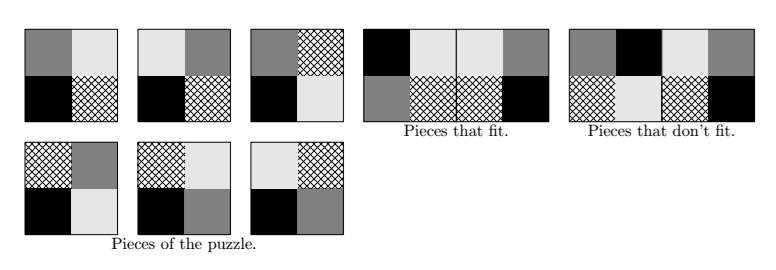
\includegraphics[scale=0.5]{24OMM1.jpg}
    \end{center}
\end{problem}

\problemdiff{2}
\begin{problem}
 %   [OMMEB 2017/N3/10]
    Encuentra todos los números de tres cifras que sean cuadrados perfectos y tales que
el número que se obtiene al invertir el orden de sus cifras también sea un cuadrado
perfecto.
\end{problem}


\problemdiff{3}
\begin{problem}
 % [OMM 2021/1] 
Los números positivos y distintos $a_1,a_2,a_3$ son tres términos consecutivos de una progresión aritmética, y de la misma manera, los números positivos y distintos $b_1,b_2,b_3$ son tres términos consecutivos de una progresión aritemética. ¿Es posible usar tres segmentos con longitudes $a_1,a_2,a_3$ como bases y otros tres segmentos con longitudes $b_1,b_2,b_3$ como alturas (en algún orden), para construir tres rectángulos con la misma área?.
\end{problem}


\problemdiff{3}

\begin{problem} %[ORO 2025/1]
    Find all thirds of three-digit numbers $abc$, $def$ and $ghi$ such that they are consecutive and that in the list formed by the digits $a, b, c, d, e, f, g, h, i$ there are no digits that appear the same number of times.
\end{problem}


\problemdiff{3}

\begin{problem}
% [OMM 2012/4] 
A cada entero positivo se le aplica el siguiente proceso: al número se le resta la suma de sus digitos, y el resultado se divide entre 9. Por ejemplo, el resultado del proceso aplicado a 938 es 102, ya que $(938-(9+3+8)/9=102)$. Aplicado dos veces el proceso a 938 se llega a 11, aplicando tres veces se llega a 1, y aplicado cuatro veces se llega al 0. Cuando a un entero positivo $n$ se le aplica el proceso una o varias veces, se termina en 0. Al número al que se llega antes de llegar al cero, lo llamamos la casa de $n$. ¿Cuántos numeros menores que 26000 tienen la misma casa que el 2012?
\end{problem}



\problemdiff{3.5}
\begin{problem}
   % [OMM 2022/1] 
    Un número $x$ es Tlahiuca si existen primos positivos distintos $p_1,p_2,\dots,p_k$ tales que 
\[x=\frac{1}{p_1}+\frac{1}{p_2}+\cdots+\frac{1}{p_k}.\]
Deterimina el mayor número Tlahuica $x$ que satisface las dos siguientes propiedades:
 \begin{itemize} 
 \item  $0< x < 1$. 
 \item  Existe un número entero $0< m\leq 2022$ tal que $mx$ es un número entero. 
 \end{itemize} 
\end{problem}

\problemdiff{4}

\begin{problem} %[ORO 2025/5]
Let $n$ be an integer positive. Let $s(n)$ be the sum of the digits of $n$. We say that $n$ is powerful if it is a square and $[1+2+\dots+s(\sqrt{n})]^2=n$. For example, 2025 es a powerful number, beacuse $2025=45^2=(1+2+\dots+9)^2$. Find all powerful numbers.
\end{problem}


\problemdiff{5}

\begin{problem} % [OMM 2024/5]
    Sean $A$ y $B$ conjuntos infinitos de reales positivos tales que:
    \begin{itemize}
        \item Para cualquier par de elementos $u \geq v$ de $A$, se cumple que $u+v$ es un elemento de $B$.
        \item Para cualquier par de elementos $s>t$ de $B$ se cumple que $s-t$ es un elemento de $A$. 
    \end{itemize}
    Prueba que $A=B$ o existe un número real $r$ tal que $B=\{ 2r,3r,4r,5r,\ldots \}$.
\end{problem}

\section{Tenga pa que se entretenga}

\problemdiff{5}
\begin{problem}
     % [IMO 2025/4]
    	A proper divisor of a positive integer $N$ is a positive divisor of $N$ other than $N$ itself.

The infinite sequence $a_1, a_2, \cdots$ consists of positive integers, each of which has at least three proper divisors. For each $n\geq 1$, the integer $a_{n+1}$ is the sum of the three largest proper divisors of $a_n$.

Determine all possible values of $a_1$.
\end{problem}

\problemdiff{6}
\begin{problem}
   % [IMO 2012/4]
    Find all functions $f:\mathbb Z\rightarrow \mathbb Z$ such that, for all integers $a,b,c$ that satisfy $a+b+c=0$, the following equality holds:
\[f(a)^2+f(b)^2+f(c)^2=2f(a)f(b)+2f(b)f(c)+2f(c)f(a).\]
\end{problem}

\problemdiff{6}
\begin{problem} % [Mercor]
    Adán y Olga están jugando un juego, olga tiene $n$ cajas, Adán infinitas pelotas. En cada ronda, Adán escoge un entero positivo $k$ que no haya escogido antes y le da $k$ pelotas a Olga, Olga pone esas $k$ pelotas en una misma caja de su elección, Olga no puede escoger dos veces seguidas la misma caja.
Adán gana si en algún punto logra que haya dos cajas con la misma cantidad (positiva) de pelotas. Para cuáles $n$ puede ganar Adán sin importar como juegue Olga?
\end{problem}



\end{document}